\newpage
\section{Home Page}

\label{Home Page}
\begin{figure}[ht]
	\centering
	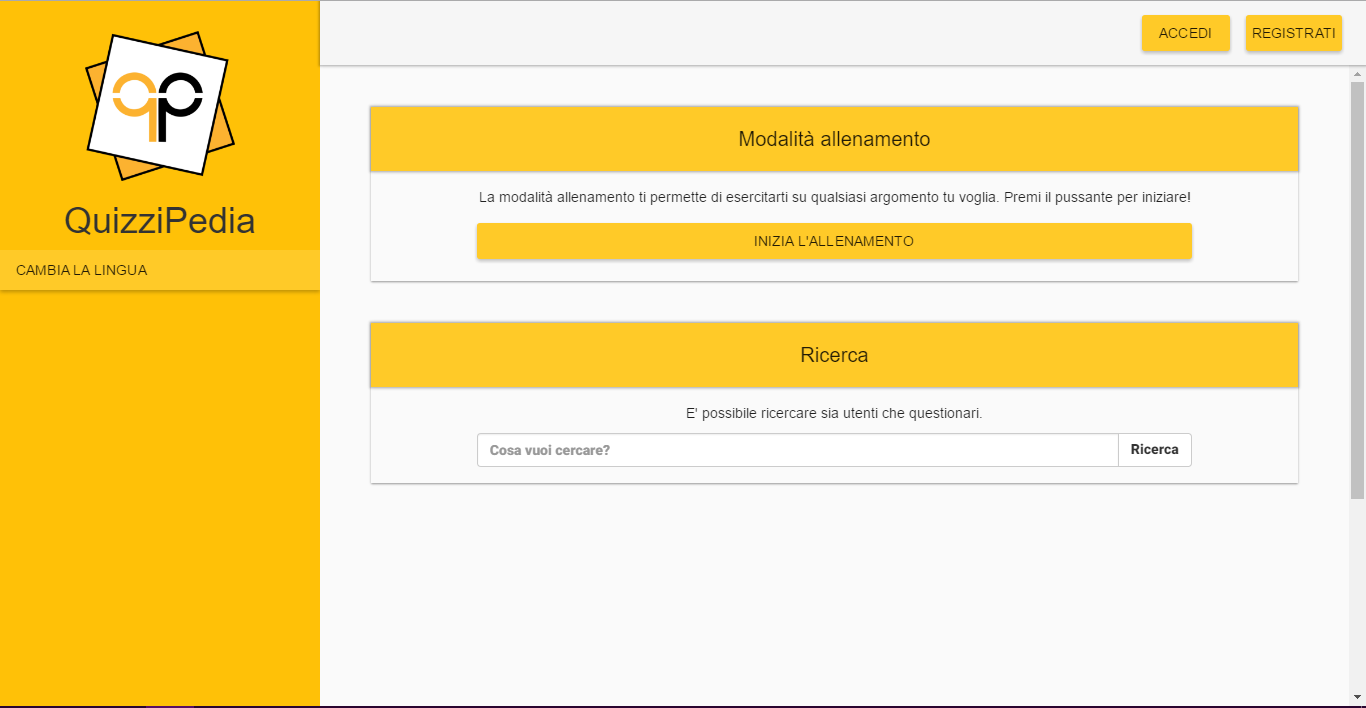
\includegraphics[scale=0.43]{img/homePage.png}
	\caption{Home Page}
\end{figure}
\FloatBarrier

L'Home Page di QuizziPedia presenta all'utente non ancora registrato le seguenti possibilità di utilizzo:
\begin{itemize}
	\item Registrazione;
	\item Autenticazione;
	\item Modalità allenamento;
	\item Ricerca utenti e questionari.
\end{itemize}
Le funzionalità \textit{Modalità allenamento} e \textit{Ricerca utenti e questionari} non necessitano di iscrizione al servizio, perciò l'utente non autenticato sarà libero di allenarsi in uno degli argomenti proposti e di ricercare i questionari e gli utenti presenti nel sistema.

\newpage
\subsection{Registrazione}

\label{Registrazione}
\begin{figure}[ht]
	\centering
	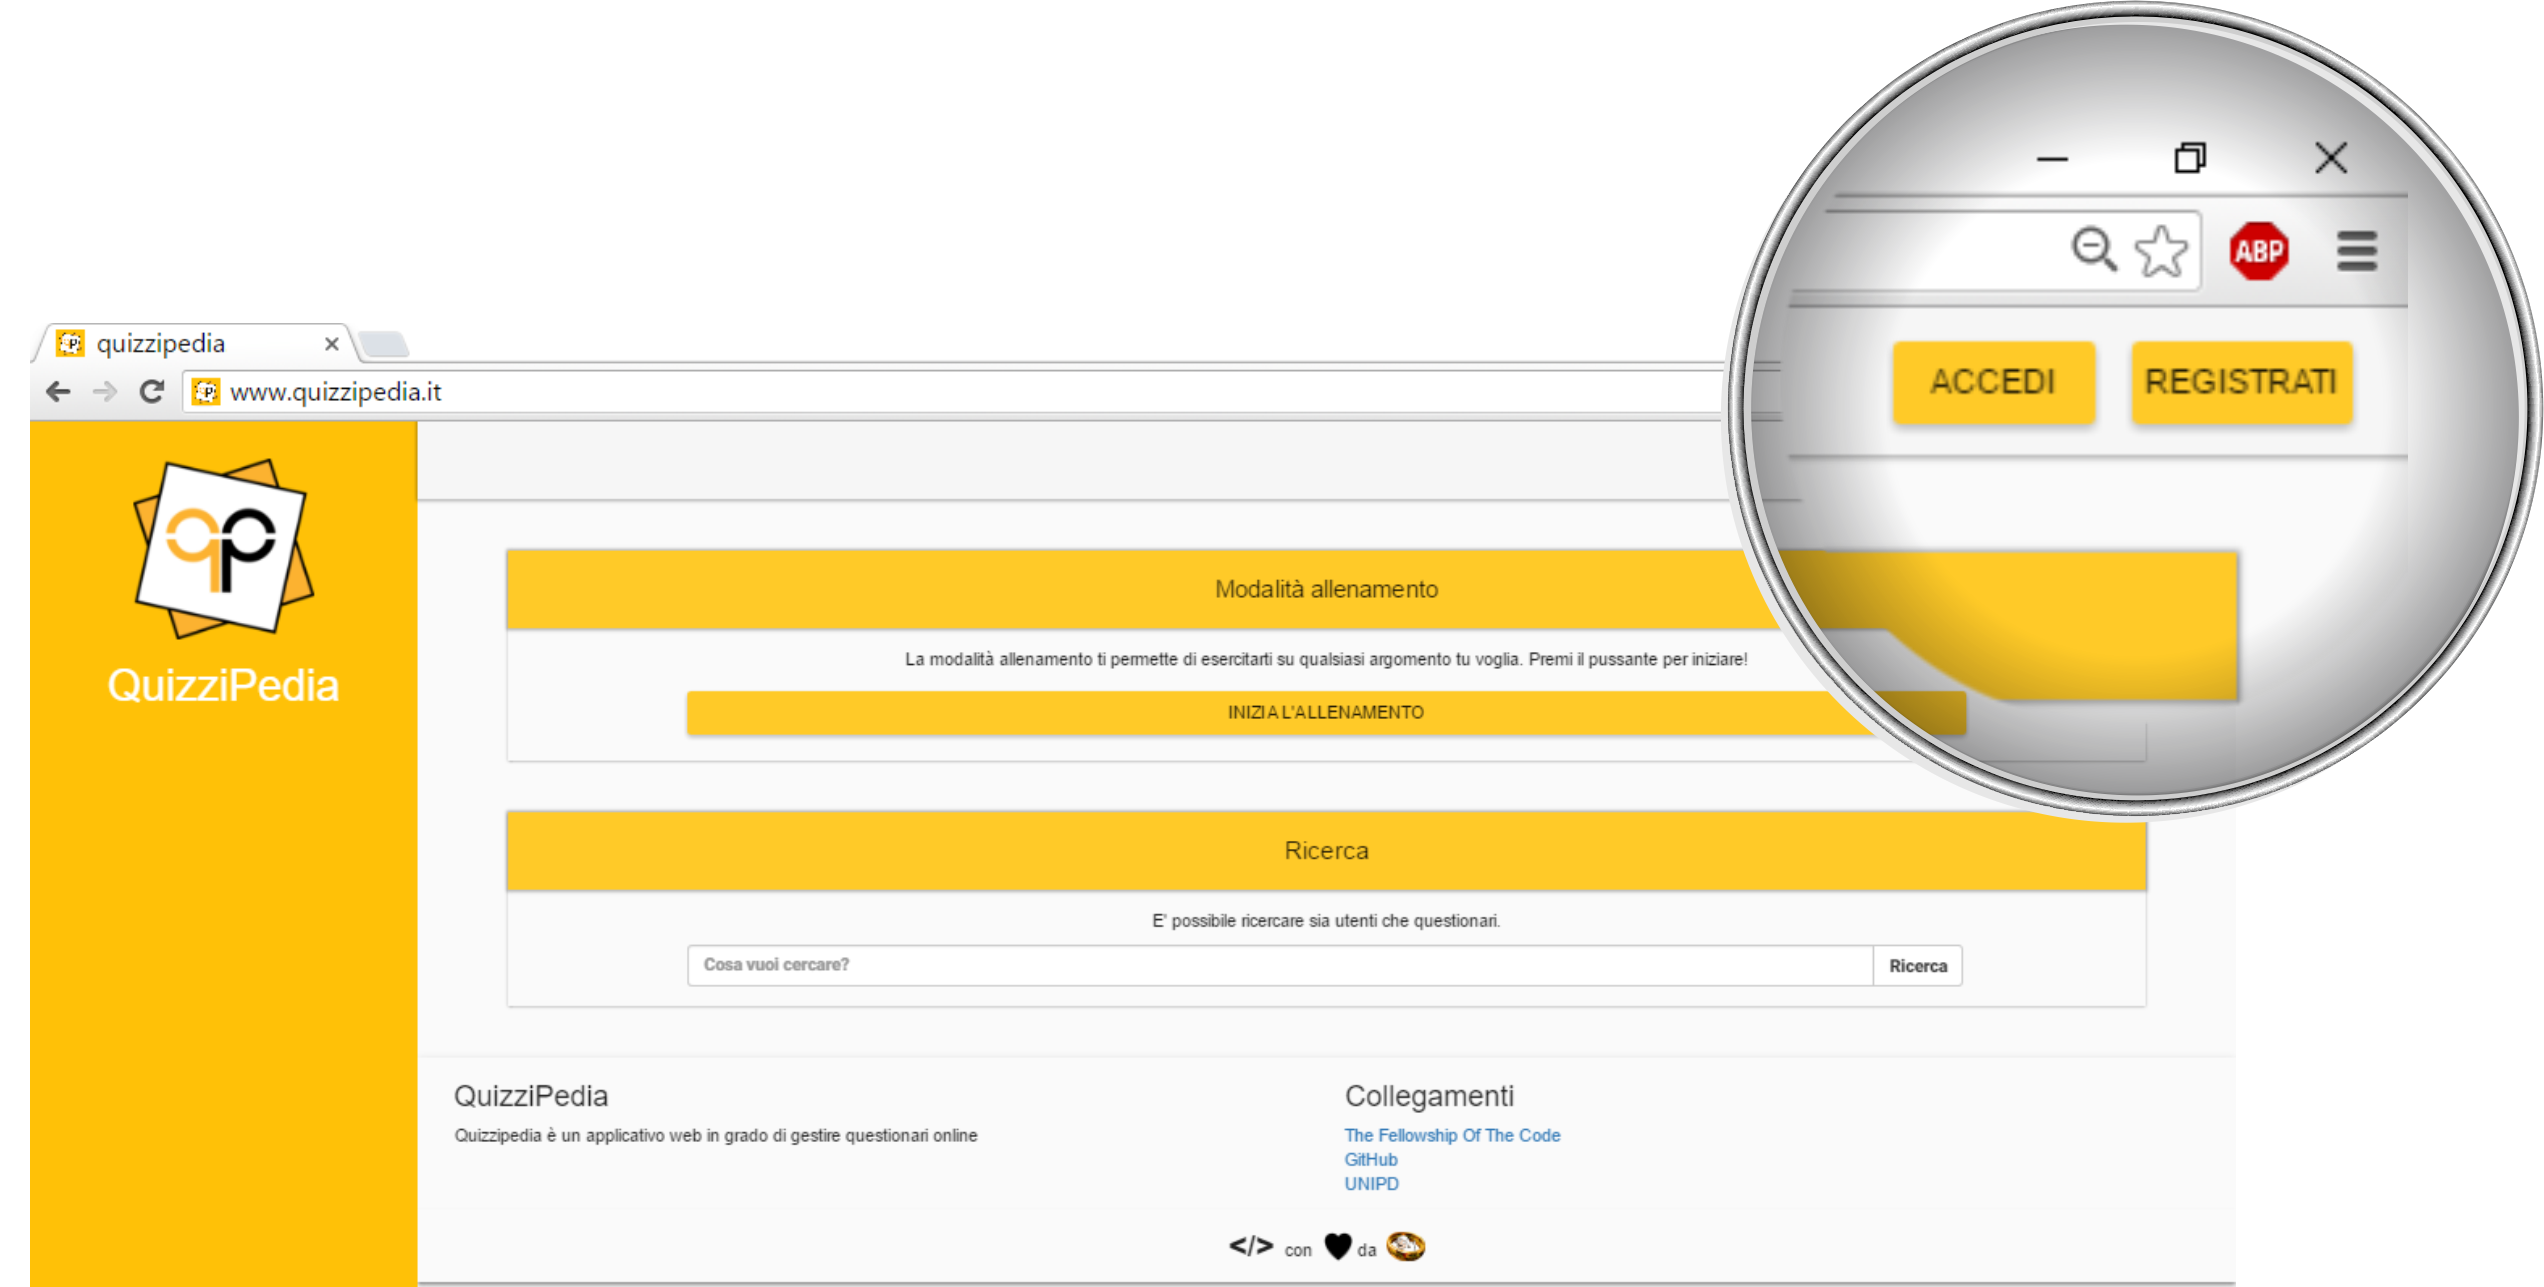
\includegraphics[scale=0.80]{img/vai_registrazione.png}
	\caption{Vai a Registrazione}
\end{figure}
\FloatBarrier

All'interno dell'Home Page è possibile accedere alla sezione \textit{Registrazione}. Una volta cliccato sul bottone apposito verrà presentata la seguente pagina:

\label{Registrazione_1}
\begin{figure}[ht]
	\centering
	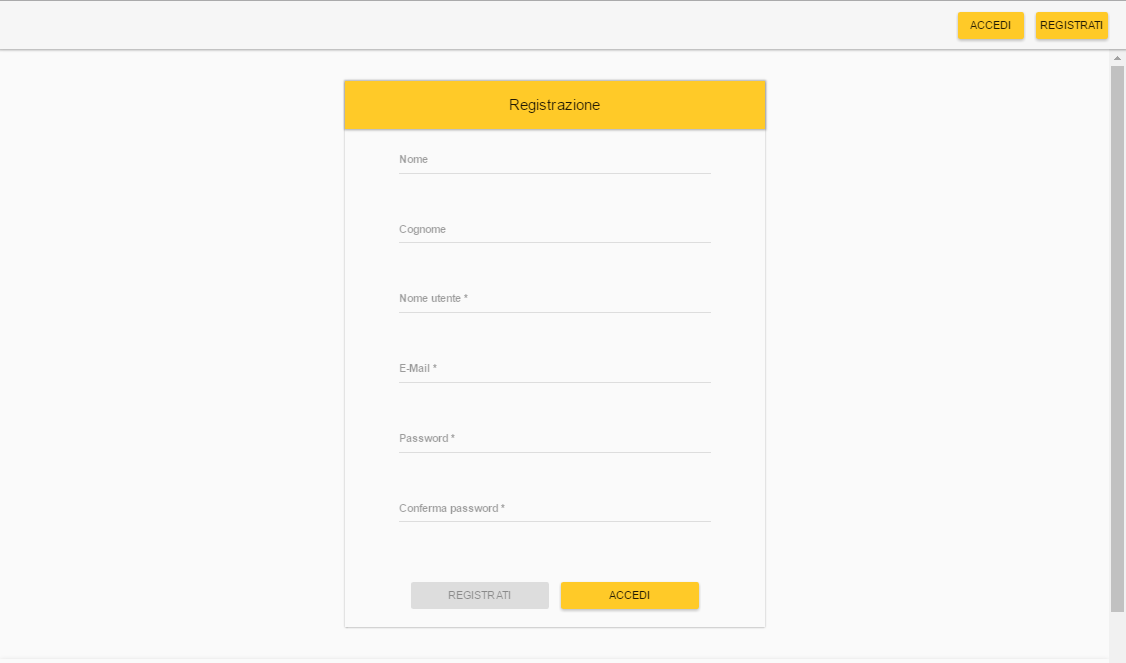
\includegraphics[scale=0.45]{img/registrazione.png}
	\caption{Registrazione}
\end{figure}
\FloatBarrier

L'utente per registrarsi deve obbligatoriamente compilare i seguenti campi:
\begin{itemize}
	\item Nome utente;
	\item E-mail;
	\item Password;
	\item Conferma password.
\end{itemize}
dove il campo \textit{Conferma password} deve essere identico al campo \textit{Password}, il quale deve avere almeno 8 caratteri. Compilati correttamente tutti i campi, il bottone \textit{Registrati}, prima disabilitato, permette di registrarsi effettuando un redirect alla pagina di autenticazione.  

\newpage
\subsection{Autenticazione}

\label{Autenticazione}
\begin{figure}[ht]
	\centering
	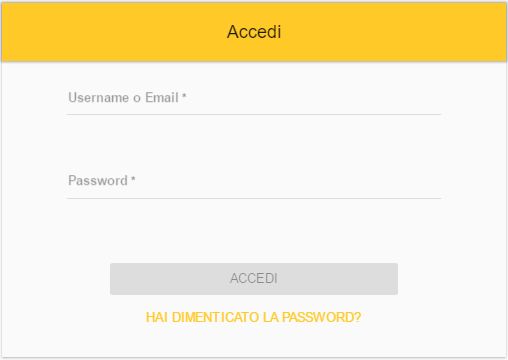
\includegraphics[scale=0.55]{img/autenticazione.png}
	\caption{Autenticazione}
\end{figure}
\FloatBarrier

Effettuata la registrazione è possibile autenticarsi al sistema. Compilati correttamente i campi \textit{Username o E-mail} e \textit{Password} il bottone \textit{Accedi} viene abilitato dando al possibilità di autenticarsi. Se l'utente non ricorda più la propria password personale è possibile cliccare sulla stringa \textit{HAI DIMENTICATO LA PASSWORD?} per recuperarla. Verrà presentata la seguente pagina:

\label{RecuperoPassword}
\begin{figure}[ht]
	\centering
	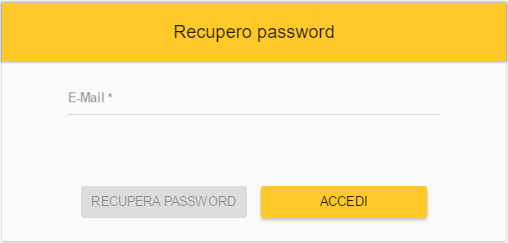
\includegraphics[scale=0.40]{img/recupero_password.png}
	\caption{Recupero Password}
\end{figure}
\FloatBarrier

la quale permette di recuperare la password inserendo la propria mail nell'apposito campo. La password sarà all'interno della mail che il sistema invierà all'indirizzo di posta elettronica inserito.  

\subsection{Modalità allenamento}
\subsection{Ricerca utenti e questionari}